\documentclass[
	a4paper,
	oneside,
	BCOR = 10mm,
	DIV = 12,
	12pt,
	headings = normal,
]{scrartcl}

%%% Length calculations
\usepackage{calc}
%%%

%%% Support for color
\usepackage{xcolor}
\definecolor{lightblue}{HTML}{03A9F4}
\definecolor{red}{HTML}{F44336}
%%%

%%% Including graphics
\usepackage{graphicx}
%%%

%%% Font selection
\usepackage{fontspec}

\setromanfont{STIX Two Text}[
	SmallCapsFeatures = {LetterSpace = 8},
]

\setsansfont{IBM Plex Sans}[
	Scale = MatchUppercase,
]

\setmonofont{IBM Plex Mono}[
	Scale = MatchUppercase,
]
%%%

%%% Math typesetting
\usepackage{amsmath}

\usepackage{unicode-math}
\setmathfont{STIX Two Math}

\usepackage{IEEEtrantools}
%%%

%%% List settings
\usepackage{enumitem}
\setlist[enumerate]{
	label*      = {\arabic*.},
	left        = \parindent,
	topsep      = 0\baselineskip,
	parsep      = 0\baselineskip,
	noitemsep, % override itemsep
}
% List settings for levels 2–4
\setlist[enumerate, 2, 3, 4]{
	label*      = {\arabic*.},
	left        = 0em,
	topsep      = 0\baselineskip,
	parsep      = 0\baselineskip,
	noitemsep, % override itemsep
}

\setlist[itemize]{
	label       = {—},
	left        = \parindent,
	topsep      = 0\baselineskip,
	parsep      = 0\baselineskip,
	itemsep     = 1\baselineskip,
	noitemsep, % override itemsep
}

\setlist[itemize, 2, 3, 4]{
	label       = {—},
	left        = 0em,
	topsep      = 0\baselineskip,
	parsep      = 0\baselineskip,
	itemsep     = 1\baselineskip,
	noitemsep, % override itemsep
}

\setlist[description]{
	font        = {\rmfamily\upshape\bfseries},
	topsep      = 1\baselineskip,
	parsep      = 0\baselineskip,
	itemsep     = 0\baselineskip,
}

%%%

%%% Structural elements typesetting
\setkomafont{pagenumber}{\rmfamily\upshape}
\setkomafont{disposition}{\rmfamily\bfseries}

% Sectioning
\RedeclareSectionCommand[
	beforeskip = -1\baselineskip,
	afterskip  = 1\baselineskip,
	font       = {\normalsize\bfseries\scshape},
]{section}

\RedeclareSectionCommand[
	beforeskip = -1\baselineskip,
	afterskip  = 1\baselineskip,
	font       = {\normalsize\bfseries\itshape},
]{subsection}

\RedeclareSectionCommand[
	beforeskip = -1\baselineskip,
	afterskip  = 1\baselineskip,
	font       = {\normalsize\bfseries},
]{subsubsection}

\RedeclareSectionCommand[
	beforeskip = -1\baselineskip,
	afterskip  = -0.5em,
	font       = {\normalsize\mdseries\scshape\addfontfeatures{Letters = {UppercaseSmallCaps}}},
]{paragraph}
%%%

%%% Typographic enhancements
\usepackage{microtype}
%%%

%%% Language-specific settings
\usepackage{polyglossia}
\setmainlanguage{ukrainian}
\setotherlanguages{english}
%%%

%%% Captions
\usepackage{caption}
\usepackage{subcaption}

%\DeclareCaptionLabelFormat{closing}{#2)}
%\captionsetup[subtable]{labelformat = closing}

%\captionsetup[subfigure]{labelformat = closing}

\captionsetup[table]{
	aboveskip = 0\baselineskip,
	belowskip = 0\baselineskip,
}

\captionsetup[figure]{
	aboveskip = 1\baselineskip,
	belowskip = 0\baselineskip,
}

\captionsetup[subfigure]{
	labelformat = simple,
	labelformat = brace,
}
%%%

%%% Hyphenated ragged typesetting
\usepackage{ragged2e}
%%%

%%% Table typesetting
\usepackage{booktabs}
\usepackage{longtable}

\usepackage{multirow}

\usepackage{array}
\newcolumntype{v}[1]{>{\RaggedRight\arraybackslash\hspace{0pt}}p{#1}}
\newcolumntype{b}[1]{>{\Centering\arraybackslash\hspace{0pt}}p{#1}}
\newcolumntype{n}[1]{>{\RaggedLeft\arraybackslash\hspace{0pt}}p{#1}}
%%%

%%% Drawing
\usepackage{tikz}
\usepackage{tikzscale}
\usetikzlibrary{positioning}
\usetikzlibrary{arrows.meta} % Stealth arrow tips

% Drawing forests and trees
\usepackage{forest}

\usepackage{tikz-uml}
%%%

%%% SI units typesetting
\usepackage{siunitx}
\sisetup{
	output-decimal-marker = {,},
	exponent-product      = {\cdot},
	inter-unit-product    = \ensuremath{{} \cdot {}},
	per-mode              = symbol,
}
%%%

% Code Highlighting
\usepackage{minted}
\setmintedinline{
	style = bw,
	breaklines,
}

\newminted[bashterm]{bash}{%
	autogobble,%
	style=bw,%
	breaklines,%
}

\newmintinline{bash}{%
}

\newminted[pythoncode]{python}{%
	autogobble,%
	style=bw,%
	breaklines,%
}

\newmintinline{python}{%
}

%%% Framing code listings
\usepackage{tcolorbox}
\tcbuselibrary{breakable}
\tcbuselibrary{minted}
\tcbuselibrary{skins}

% Text file listing
\newtcblisting[
	auto counter,
	list inside, 
	number within = section,
]{listingplaintext}[3][]{%
	minted language = text,
	minted style    = bw,
	minted options  = {
		autogobble,
		linenos,
		tabsize = 4,
		breaklines,
		breakanywhere,
		fontsize = \footnotesize,
	},
	empty,
	sharp corners,
	coltitle = black,
	borderline horizontal = {1pt}{0pt}{black},
	titlerule = {0.5pt},
	titlerule style = {
		black,
	},
	toptitle = 0.3em,
	bottomtitle = 0.3em,
	before skip      = \intextsep,
	after  skip      = \intextsep,
	title            = {Лістинг \thetcbcounter: #2},
	list entry       = {\protect\numberline{\thetcbcounter}#2},
	left = 0em,
	right = 0em,
	%
	listing only,
	breakable,
	%
	label = {#3},%
}

\newtcblisting[
	use counter from = listingplaintext,
	list inside, 
	number within = section,
]{listingpython}[3][]{%
	minted language = python,
	minted style    = bw,
	minted options  = {
		autogobble,
		linenos,
		tabsize = 4,
		breaklines,
		breakanywhere,
		fontsize = \footnotesize,
	},
	empty,
	sharp corners,
	coltitle = black,
	borderline horizontal = {1pt}{0pt}{black},
	titlerule = {0.5pt},
	titlerule style = {
		black,
	},
	toptitle = 0.3em,
	bottomtitle = 0.3em,
	before skip      = \intextsep,
	after  skip      = \intextsep,
	title            = {Лістинг \thetcbcounter: #2},
	list entry       = {\protect\numberline{\thetcbcounter}#2},
	left = 0em,
	right = 0em,
	%
	listing only,
	breakable,
	%
	label = {#3},
	%
	#1%
}

\newtcbinputlisting[
	use counter from = listingplaintext,
	list inside,
	number within = section
]{\inputpython}[4][]{%
	minted language = python,
	minted style    = bw,
	minted options  = {
		autogobble,
		linenos,
		tabsize = 4,
		breaklines,
		breakanywhere,
		fontsize = \footnotesize,
	},
	empty,
	sharp corners,
	coltitle = black,
	borderline horizontal = {1pt}{0pt}{black},
	titlerule = {0.5pt},
	titlerule style = {
		black,
	},
	toptitle = 0.3em,
	bottomtitle = 0.3em,
	before skip      = \intextsep,
	after  skip      = \intextsep,
	title            = {Лістинг \thetcbcounter: #3},
	list entry       = {\protect\numberline{\thetcbcounter}#3},
	left = 0em,
	right = 0em,
	%
	listing file={#2},
	listing only,
	breakable,
	%
	label = {#4}
}

% Linux command-line listing
\newtcblisting{linuxterm}%
{%
	% Syntax highlighing options
	listing only,%
	minted language = bash,%
	minted options={%
		autogobble,%
		linenos%
	},%
	% Presentation options
	empty,%
	%% Margins
	sharp corners,%
	toptitle = 0.0em,%
	bottomtitle = 0.0em,%
	left = 0em,%
	right = 0em,%
	before skip = \intextsep,%
	after skip = \intextsep,%
}

\newtcblisting{linuxtermout}%
{%
	% Syntax highlighing options
	listing only,%
	minted language = text,%
	minted options={%
		autogobble,%
		linenos%
	},%
	% Presentation options
	empty,%
	%% Margins
	sharp corners,%
	toptitle = 0.0em,%
	bottomtitle = 0.0em,%
	left = 0em,%
	right = 0em,%
	before skip = \intextsep,%
	after skip = \intextsep,%
}

% Dockerfile listings
\newtcblisting[
	use counter from = listingplaintext,
	list inside, 
	number within = section,
]{listingdocker}[3][]{%
	minted language = dockerfile,
	minted style    = bw,
	minted options  = {
		autogobble,%
		linenos,
		tabsize = 4,
		breaklines,
		breakanywhere,
		fontsize = \footnotesize,
	},
	empty,
	sharp corners,
	coltitle = black,
	borderline horizontal = {1pt}{0pt}{black},
	titlerule = {0.5pt},
	titlerule style = {
		black,
	},
	toptitle = 0.3em,
	bottomtitle = 0.3em,
	before skip      = \intextsep,
	after  skip      = \intextsep,
	title            = {Лістинг \thetcbcounter: #2},
	list entry       = {\protect\numberline{\thetcbcounter}#2},
	left = 0em,
	right = 0em,
	%
	listing only,
	breakable,
	%
	label = {#3},%
}

% Docker Compose listings
\newtcblisting[
	use counter from = listingplaintext,
	list inside, 
	number within = section,
]{listingdockercompose}[3][]{%
	minted language = yaml,
	minted style    = bw,
	minted options  = {
		autogobble,%
		linenos,
		tabsize = 4,
		breaklines,
		breakanywhere,
		fontsize = \footnotesize,
	},
	empty,
	sharp corners,
	coltitle = black,
	borderline horizontal = {1pt}{0pt}{black},
	titlerule = {0.5pt},
	titlerule style = {
		black,
	},
	toptitle = 0.3em,
	bottomtitle = 0.3em,
	before skip      = \intextsep,
	after  skip      = \intextsep,
	title            = {Лістинг \thetcbcounter: #2},
	list entry       = {\protect\numberline{\thetcbcounter}#2},
	left = 0em,
	right = 0em,
	%
	listing only,
	breakable,
	%
	label = {#3},%
}

% Customize minted line numbers
\renewcommand{\theFancyVerbLine}{\ttfamily\scriptsize\arabic{FancyVerbLine}}

%%%

%%% Bibliography
\usepackage[
	style    = gost-numeric,
	language = auto,
	autolang = other,
	sorting  = none,
	maxcitenames = 2,
]{biblatex}
\addbibresource{y03s02-practice-01-report-bibliography.bib}
%%%

%%% Links and hyperreferences
\usepackage{hyperref}
\hypersetup{
	bookmarksnumbered = true,
	colorlinks      = false,
	linkbordercolor = red,
	urlbordercolor  = lightblue,
	pdfborderstyle  = {/S/U/W 1.5},
}
%%%

%%% Length adjustment

% Set baselineskip, default is 14.5 pt
\linespread{1.068966} % ~15.5 pt
\setlength{\emergencystretch}{1em}
\setlength{\parindent}{1.5em}
\newlength{\gridunitwidth}
\setlength{\gridunitwidth}{\textwidth / 12}
%%%

%%% Custom commands
\newcommand{\allcaps}[1]{%
	{%
		\addfontfeatures{%
			Letters = UppercaseSmallCaps,
			LetterSpace = 8,%
			Kerning = Off%
		}%
		#1%
	}%
}
\newcommand{\makeallcaps}[1]{%
	\allcaps{\MakeUppercase{#1}}
}
\newcommand{\filename}[1]{\texttt{#1}}
\newcommand{\progname}[1]{\texttt{#1}}
\newcommand{\commandname}[1]{\texttt{#1}}
\newcommand{\modulename}[1]{\texttt{#1}}
\newcommand{\transeng}[1]{{англ.}~\textit{\textenglish{#1}}}
\newcommand{\elemtitle}[1]{%
	{\centering%
		\makeallcaps{#1}%
		\par
	}
}
\newcommand{\elemtitleext}[2]{%
	{\centering%
		\makeallcaps{#1}\\%
		#2%
		\par
	}
}
\newcommand{\blank}[1]{\rule[-0.0em]{#1}{0.4pt}}
\newcommand{\lastblank}{\hrulefill}
%%%

%%% Custom math commands
\newcommand{\longvar}[1]{\mathit{#1}}
%%%

\begin{document}

\begin{titlepage}
		\begin{center}
			Міністерство освіти і~науки України\\
			Національний авіаційний університет\\
			Факультет кібербезпеки, комп'ютерної і~програмної інженерії\\
			Кафедра комп'ютеризованих систем управління

			\vspace{\fill}
				Звіт\\
				з~проектно-технологічної практики

			\vspace{\fill}

			\begin{flushleft}
				студента 3~курсу \allcaps{СП}-325~групи\\
				напряму~123~«Комп'ютерна інженерія»\\
				Клокуна Владислава Денисовича\\[1\baselineskip]

				База практики: \allcaps{ТОВ} «Смарт Медіа Інвест»\\[1\baselineskip]

				Керівник практики:\\
				від університету — старший викладач Кашкевич Іван Фуркатович\\
				від бази практики — керівник проектів Чезганов Олександр Сергійович\\
			\end{flushleft}
			
			% \vspace{\fill}

			Київ 2019
		\end{center}
	\end{titlepage}

	\thispagestyle{empty}%
	{%
		\setlength{\parindent}{0em}%
		\setlength{\parskip}{1\baselineskip}%
		Підстава для~проходження практики: робочий навчальний план №~РС-4-6.05010202/12 підготовки фахівців за~напрямом підготовки 6.050102~«Комп'\-ю\-те\-рна інженерія», договір на~проведення практики між університетом та~\allcaps{ТОВ} «Смарт Медіа Інвест», наказ ректора №~687/ст~від 10.04.2019.

		% \vspace{1\baselineskip}
		Термін проходження практики: з~03.06.2019 по~23.06.2019

		% \vspace{1\baselineskip}
		Індивідуальні завдання: розробити програмний продукт~— чат-бота для~платформи~\textenglish{Telegram}.

		\elemtitleext{Відмітка}{про проходження практики}
		Прибув на~базу практики\\
		«\blank{3em}» \blank{9em} 2019~р. (підпис) \lastblank{} М.\,П.

		% \vspace{1\baselineskip}
		Вибув з~бази практики\\
		«\blank{3em}» \blank{9em} 2019~р. (підпис) \lastblank{} М.\,П.

		\elemtitle{Календарний план-графік практики}
		\begin{tabular}{
			|n{1\gridunitwidth - 2\tabcolsep}
			|v{6.5\gridunitwidth - 2\tabcolsep}
			|n{2.25\gridunitwidth - 2\tabcolsep}
			|n{2.25\gridunitwidth - 2\tabcolsep}
			|
		}
			\hline
				\multirow{2}{\linewidth}{№ п/п} & \multirow{2}{*}{Об'єкт практики та~види робіт} & \multicolumn{2}{c|}{Термін виконання}\\
					\cline{3-4}
					&  & початок & закінчення\\
			\hline
				 1 & Знайомство з~інфраструктурою і~забезпеченням організації & 03.06.2019 & 05.06.2019 \\
				\hline
				 2 & Постановка і~аналіз задачі. Вибір необхідних інструментів для~розробки. Затвердження специфікації & 06.06.2019 & 07.06.2019 \\
				\hline
				 3 & Розробка програмного продукту & 10.06.2019 & 14.06.2019 \\
				\hline
				 4 & Розробка рішення для~розгортання програми & 17.06.2019 & 18.06.2019 \\
				\hline
				 5 & Тестування розробленого програмного продукту & 19.06.2019 & 21.06.2019 \\
			\hline
		\end{tabular}

		Керівник практики від університету: \lastblank
	}

	% Finish introductory pages
	\newpage
	\tableofcontents

	\newpage
	\section{Характеристика бази практики}
		\subsection{Загальні відомості про організацію}
			Організація \allcaps{ТОВ}~«Смарт Медіа Інвест» зареєстрована за~адресою 47201, Тернопільська~область, Зборівський~район, місто~Зборів, вулиця~Б.\,Хмельницького. За~класифікатором видів економічної діяльності вона є~рекламним агентством, займається створенням, запуском, супроводом, просуванням і~підтримкою медіапроектів у~соціальних мережах на~кшталт «Вконтакте», «\textenglish{Instagram}» і~«\textenglish{Telegram}».
			
		\subsection{Сфера діяльності}
			Щоб підтримувати медіапроект, необхідно збирати, створювати, оформлювати і~публікувати інформацію, на~якій він спеціалізується, розважати користувачів проекту, а~також тримати його у~належному стані. Для досягнення цих цілей і~покращення результатів використовують різні інструменти: для~розваги користувачів~— мультимедійні матеріали і~інтерактивні заходи, для~підтримки проекту~— спеціальні програмні продукти.
		
		За~кожну зі~складових відповідають певні структурні підрозділи, які~тісно взаємодіють між собою. Пошуком і~створенням інформації, розробкою ідей, креативу, а~також інтерактивних заходів займаються редактори. Мультимедійні матеріали для~оформлення розроблених ідей надають дизайнери. За~створення і~запуск інструментів, необхідних для~організації інтерактивних розважальних заходів і~підтримки медіапроектів, відповідають розробники. Крім цього, розробники відповідають за~налаштування і~підтримку апаратно-програмної інфраструктури, яка~необхідна для~правильної роботи вже запущених продуктів, у~справному стані.
		
		Інструменти, створенням і~запуском яких займаються розробники, можна класифікувати так:
		\begin{itemize}
			\item розважальні інструменти:
				\begin{itemize}
					\item чат-боти,
					\item боти-коментатори,
				\end{itemize}
			\item супровідні інструменти:
				\begin{itemize}
					\item очищувачі,
					\item спеціалізовані сценарії (живі обкладинки тощо),
					\item інструменти збору статистики.
				\end{itemize}
		\end{itemize}
		Щоб зрозуміти, що~входить в~обов'язки розробників, розглянемо кожен клас цих інструментів детальніше. \emph{Розважальні інструменти} призначені для~того, щоб~розважити користувача, безпосередньою взаємодією з~ним. Прикладом розважального інструменту є~\emph{чат-бот}~— програмний продукт, який~веде діалог (чат) з~користувачем відповідно до~заданого сценарію або~специфікації. Наприклад, за~допомогою чат-бота можна реалізувати текстову пригоду, головним героєм якого буде кожен окремий користувач, організувати лотерею або~віртуального помічника, який~відповідатиме на~питання користувача.

		\emph{Бот-коментатор}~— це~програмний продукт, який~додає коментарі у~спеціальних дошках для~обговорення у~соціальних мережах залежно від певної умови. Наприклад, якщо користувач залишає коментар до~запису про товар, в~якому питає про деталь, відому боту-коментатору, цей бот може залишити коментар з~відповіддю на~поставлене питання. 

		Наступною категорією є~\emph{супровідні інструменти}, тобто інструменти, призначені для~автоматизованої підтримки представництв медіапроекту у~певному стані. Першим представником супровідних інструментів є~\emph{очищувач}~— програмний продукт який~очищує ту~чи~іншу складову присутності медіапроекту у~соціальній мережі: записи на~дошці обговорень та~її~коментарі, зміст фото-, аудіо- і~відеоальбомів тощо.

		\emph{Спеціалізований сценарій} (або~\emph{скрипт})~— це~програмний продукт, який~виконує різноманітні вузькоспеціалізовані дії в~залежності від свого призначення. Поширеним прикладом спеціалізованого сценарію є~«жива обкладинка»~— програмний продукт, який~змінює обкладинку представництва медіапроекту у~соціальній мережі в~залежності від певних параметрів: кількості записів, створених користувачами, проведених дій, переглядів тощо.

		\emph{Інструмент збору статистики}~— це~програмний продукт, який~збирає статистику різних представництв медіапроекту у~соціальних мережах, оброблює зібрані дані та~експортує їх~у~потрібний формат. Результати роботи цих інструментів використовуються для~аналізу, відстеження і~планування стану та~життєздатності проекту, а~також для~звітності.

		Отже, як~бачимо, компанія займається повним циклом управління медіапроектами. Для цього вона використовує набір різноманітних інструментів, до~яких також входять програмні інструменти, за~створення і~запуск яких відповідає підрозділ розробників, в~якому автор проходив практику.

	\section{Зміст та~результати виконаних робіт}
		\subsection{Знайомство з~інфраструктурою і~забезпеченням організації}
			Організована у~компанії інфраструктура для~розробки програмних рішень складається з~апаратного і~програмного забезпечення, а~також віддалених сервісів. Віддалені (або~\emph{хмарні}) сервіси використовуються для~координації команди і~збереження її~напрацювань. Організація використовує такі сервіси:
			\begin{itemize}
				\item хостинг для~репозитаріїв початкового коду~\textenglish{GitHub};
				\item система організації документообігу~\textenglish{Google Suite: Docs, Sheets} і~{Slides};
				\item дошка завдань~\textenglish{Trello}.
			\end{itemize}

			Хостинг для~репозитаріїв початкового коду~\textenglish{GitHub} потрібен, щоб~зберігати і~відстежувати версії початкового коду усіх програмних продуктів і~інструментів, які~створюються і~використовуються в~організації. Система організації документообігу~\textenglish{Google Suite} використовується для~звітності та~обміну документами між працівниками компанії. На~дошці завдань~\textenglish{Trello} відстежують завдання, які~зараз поставлені перед працівниками, і~оцінюють їх~завантаженість, щоб~планувати наступні дії.
			
			До~апаратного забезпечення входить виділений сервер, розташований за~межами компанії, на~якому встановлене програмне забезпечення, необхідне для~розробки продуктів, якими користується організація, зокрема:
			\begin{itemize}
				\item операційна система~\textenglish{\allcaps{GNU}/Linux Ubuntu \allcaps{LTS}};
				\item веб-сервер~\textenglish{Nginx};
				\item система керування базами даних~\textenglish{MongoDB};
				\item інтерпретатор мови програмування~\textenglish{Python};
				\item система управління контейнерами~\textenglish{Docker}.
			\end{itemize}
			
			Розглянемо вищезазначене програмне забезпечення детальніше. Операційна система~\textenglish{\allcaps{GNU}/Linux Ubuntu \allcaps{LTS}} дозволяє встановити всі засоби, необхідні для~правильної роботи потрібних продуктів, наприклад, \textenglish{Docker Server Community Edition}. На~робочій машині встановлена серверна версія дистрибутиву, що~дозволяє зменшити обсяг пам'яті, який~займає система, бо~в~ній встановлюється лише набір мінімально необхідних компонентів. Позначка~\textenglish{\allcaps{LTS}~(Long-Term Support)} означає, що~ця~версія дистрибутиву буде підтримуватись тривалий час, тобто в~разі виникнення проблем з~системою можна розраховувати на~необхідну підтримку протягом декількох років з~моменту випуску даної версії.

			На~операційній системі встановлений веб-сервер~\textenglish{Nginx}, необхідний для~запуску програмних продуктів, які~надають послуги в~мережі Інтернет, зокрема веб-додатків та~веб-сайтів. На~одному сервері водночас можуть працювати одразу декілька продуктів, тому веб-сервер виступає як~зворотний проксі~(\transeng{reverse proxy}), тобто отримує запити від зовнішніх клієнтів і~перенаправляє їх~на~інші, локальні веб-сервери.

			Система керування базами даних~\textenglish{MongoDB} використовується для~збереження і~управління постійними відносно структурованими даними, які~створюються під~час роботи веб-додатків. 

			Основною мовою програмування для~розробки продуктів в~організації є~\textenglish{Python}, тому на~сервері встановлений її~інтерпретатор. З~його допомогою розробники створюють модулі та~пакети на~мові програмування~\textenglish{Python} і~запускають їх.

			Щоб зручно розгортати продукти і~запускати їх~в~ізольованому середовищі, яке можна точно відтворити на~будь-якій сумісній платформі, використовують систему управління контейнерами~\textenglish{Docker}. %Вона дозволяє створити з~компонентів програмного продукту спеціальні об'єкти, які~будуть точно відтворюватись і~запускатись на~усіх платформах~\textenglish{Docker}.

		\subsection{Постановка і~аналіз задачі}
		\label{ssec:problem-description}
			Для проходження проектно-технологічної практики була поставлена така задача: розробити чат-бота для~платформи~«\textenglish{Telegram}», який~надсилає казки своїм користувачам. Коли користувач запускає бота, він повинен привітати його і~надіслати випадкову казку. Якщо користувач просить надіслати ще, бот надсилає наступну випадкову казку. Також, бот повинен регулярно розсилати казки своїм користувачам: щодня в~певний час.
			
			Щоб наочно зобразити високорівневу функціональність бота, була розроблена \textenglish{\allcaps{UML}}-діаграма варіантів використання чат-бота~(рис.~\ref{fig:bot-diag-use-case}).

			\begin{figure}[!htbp]
				\centering
				\begin{tikzpicture}
					\tikzumlset{fill usecase=white}
					\begin{umlsystem}{Чат-бот}
						\umlusecase[x = 04, y = 00, width = 2\gridunitwidth, name = start-bot]{Підписатись на~розсилку}
						\umlusecase[x = 04, y = 02, width = 2\gridunitwidth, name = request-tale]{Отримати казку}
						\umlusecase[x = 10.5, y = 02, width = 2\gridunitwidth, name = request-tale-reg]{Отримати щоденну казку}
						\umlusecase[x = 04, y = 04.5, width = 2\gridunitwidth, name = rate-tale]{Оцінити отриману казку}
					\end{umlsystem}

					% Define actors
					\umlactor[x = 00, y = 02, name = user]{Користувач}

					\umlassoc{Користувач}{start-bot}
					\umlassoc{Користувач}{request-tale}
					\umlassoc{Користувач}{rate-tale}
					\umlinclude{request-tale}{request-tale-reg}

				\end{tikzpicture}
				\caption{Діаграма варіантів використання чат-бота}
				\label{fig:bot-diag-use-case}
			\end{figure}

			Розроблена діаграма варіантів використання допомогла затвердити вимоги до~програмного продукту з~працівниками, які~розробляли ідею даного проекту, і~знадобилась під~час розробки архітектури програмного продукту.

			Щоб проаналізувати задачу, розділимо її~на~підзадачі. В~результаті декомпозиції отримаємо таку ієрархію:
			\begin{enumerate}
				\item Регулярно надсилати випадкову казку.
				\item Обробити запит користувача:
					\begin{enumerate}
						\item Визначити тип запиту.
						\item Додати користувача в~список активних користувачів чат-бота.
						\item Дати відповідь на~запит:
							\begin{enumerate}
								\item Надіслати повідомлення-привітання.
								\item Надіслати повідомлення з~інструкцією, як~користуватись чат-ботом.
								\item Обрати випадкову казку.
								\item Надіслати текст обраної казки.
								\item Додати казку у~список казок, що~подобаються.
							\end{enumerate}
					\end{enumerate}
			\end{enumerate}

		\subsection{Вибір інструментів і~затвердження специфікації}
			Як~відомо зі~знайомства з~інфраструктурою компанії, основною мовою програмування для~створення продуктів є~\textenglish{Python}, тому для~розробки чат-бота буде використана саме вона. 

			Розглянемо діаграму варіантів використання~(рис.~\ref{fig:bot-diag-use-case}), з~якої видно, що~при взаємодії з~системою (Чат-ботом) актор (Користувач) може виконувати такі дії:
			\begin{itemize}
				\item Підписатись на~розсилку, тобто дати згоду на~те, щоб~бот працював з~користувачем, який~до~нього звертається.
				\item Отримати казку, тобто надіслати запит чат-боту, щоб~він надіслав користувачу казку. 
				\item Отримати щоденну казку, яка~є~розширенням варіанту використання «Отримати казку». Якщо користувач підписався на~розсилку, бот надсилає щоденну казку за~заданим розкладом.
				\item Оцінити отриману казку, тобто мати змогу виразити, що~казка сподобалась користувачу.
			\end{itemize}

			\subsubsection{Взаємодія з~платформою~\textenglish{Telegram}}
				Основною можливістю є~взаємодія з~чат-ботом. Він повинен працювати на~платформі~\textenglish{Telegram}, тож необхідно використати її~програмний інтерфейс~(\transeng{application programming interface, \allcaps{API}}). Програмний інтерфейс~\textenglish{Telegram}, а~тому і~робота більшості чат-ботів побудована на~основі двох дій: отримання і~обробки оновлень та~постановки запитів до~серверів~\textenglish{Telegram \allcaps{API}}.

				Отримання оновлень дозволяє зрозуміти, які~дії користувачі або~інші треті сторони проводять з~ботом. Наприклад, які~повідомлення надсилають, які~кнопки натискають та~інше. Запити дозволяють визначити, які~дії повинен провести сам чат-бот: яке повідомлення відправити у~відповідь, яку інформацію отримати або~оновити тощо.

				Щоб організувати взаємодію з~платформою~\textenglish{Telegram}, скористаємось зовнішнім пакетом~«\textenglish{Python Telegram Bot}»~(знаходиться за~адресою \url{https://github.com/python-telegram-bot/python-telegram-bot}), який~надає модулям, написаним на~мові програмування~\textenglish{Python} зручний доступ до~інтерфейсу програмування платформи~\textenglish{Telegram}. Цей модуль дозволяє отримувати оновлення за~допомогою двох методів: довгого опитування~(\transeng{long polling}) і~веб-перехоплення~(\transeng{webhook}).
				
				Метод \emph{довгого опитування}~— це~\textenglish{pull}-технологія (тобто спочатку клієнт робить запит, а~потім сервер відповідає), при використанні якої клієнт опитує сервер з~певним інтервалом. Однак, на~відміну від традиційного опитування, клієнт очікує, що~сервер може відповісти не~одразу. Натомість, якщо сервер не~має оновлень для~клієнта, він не~відсилає пусту відповідь, а~чекає, поки з'явиться оновлення або~закінчиться період опитування, і~лише тоді надсилає відповідь і~закінчує цикл «запит—відповідь».
				
				Перевагами методу довгого опитування є:
				\begin{enumerate}
					\item Можливість працювати на~будь-якому пристрої, здатному робити запити до~веб-серверів.
					\item Менша затримка на~відповідь (тобто між моментами, коли інформація з'явилась і~коли клієнт надіслав запит на~її~отримання) порівняно зі~звичайним опитуванням.
					\item Простота реалізації.
				\end{enumerate}
				Його недоліком є~більша потреба в~обчислювальних і~мережевих ресурсах, а~отже менша продуктивність і~швидкодія додатків, основаних на~ньому.

				Отже, техніку довгого опитування можна досить просто реалізувати на~більшості пристроїв, підключених до~мережі, і~вона дозволяє досить швидко отримувати оновлення, однак, під~великим навантаженням вона потребуватиме велику кількість обчислювальних і~мережевих ресурсів.

				Метод \emph{веб-перехоплення}~— це~\textenglish{push}-технологія (тобто сервер розпочинає обмін даними і~надсилає повідомлення без~попередього запиту), при використанні якої сервер надсилає запит за~вказаною адресою, як~тільки з'являється оновлення. Метод називається веб-перехопленням, тому що~за~адресою, куди надсилається запит, знаходиться веб-сервер, який~його перехоплює, оброблює і, за~потреби, дає відповідь.

				Такий метод має серйозні переваги в~області швидкодії, а~саме:
				\begin{enumerate}
					\item Найменшу затримку на~відповідь серед усіх методів.
					\item Мінімальне навантаження на~обчислювальні і~мережеві ресурси.
				\end{enumerate}
				Однак, висока продуктивність методу потребує компромісу і~має суттєвий недолік: метод веб-перехоплення важче реалізувати порівняно з~іншими, оскільки для~цього потрібні такі складові:
				\begin{itemize}
					\item сервер зі~статичною \textenglish{\allcaps{IP}}-адресою, який~може отримувати запити з~мережі Інтернет;
					\item веб-сервер з~підтримкою протоколу~\textenglish{\allcaps{TLS}~1.0} і~вище;
					\item відкриті порти 443, 80, 88 або~8443.
					\item \textenglish{\allcaps{SSL}}-сертифікат безпеки.
				\end{itemize}
				
				Отже, веб-перехоплення дозволяє отримувати оновлення одразу ж, без~потреби так чи~інакше опитувати сервер, і~економить обчислювальні ресурси. Проте, йому необхідно багато сторонніх ресурсів, що~ускладнює реалізацію, тому використовувати метод веб-перехоплення рекомендують виключно тоді, коли в~цьому є~реальна потреба~\cite{ptb-longpoll-webhooks}.

				У~завданні не~передбачена вимога високої доступності та~можливість витримати високе навантаження, крім того, апаратне забезпечення достатньо швидке, щоб~витримати відносно велику кількість користувачів, тому для~реалізації чат-бота був обраний метод довгого опитування.

			\subsubsection{Інструменти веб-додатку}
				Щоб кожен день розсилати казки користувачам, які~звернулись до~бота і~підписались на~розсилку, необхідно вести їх~облік. Хорошою практикою при розробці веб-додатків є~принцип відсутності стану: дії, які~виконує програма~— веб-додаток, не~повинні залежати від її~внутрішнього стану. Отже, облікові дані користувачів варто зберігати зовні, за~логічними межами програми.

				Так як~облікові дані користувачів будуть часто змінюватись (будуть з'я\-вля\-тись нові користувачі, оцінки тощо), для~збереження цих даних зручно використати базу даних. В~організації вже використовують систему керування базами даних~\textenglish{MongoDB}, тому для~вирішення поставленої задачі використаємо її.

				Щоб отримати доступ до~бази даних з~\textenglish{Python}-модуля, використаємо пакет~\textenglish{PyMongo}, який~надає офіційний розробник системи керування базами даних~\textenglish{MongoDB}.

			\subsubsection{Результати}
				На~основі дослідженої інформації та~проведених порівнянь для~розробки програмного продукту були обрані необхідні інструменти~(табл.~\ref{tab:chosen-tools}).

				\begin{table}[!htbp]
					\caption{Обрані інструменти}
					\label{tab:chosen-tools}
					\centering
					\begin{tabular}{
						v{5\gridunitwidth - 2\tabcolsep}
						v{7\gridunitwidth - 2\tabcolsep}
					}
						\toprule
							Призначення & Обраний інструмент\\
						\midrule
							Мова програмування & \textenglish{Python}\\
							Взаємодія з~платформою~\textenglish{Telegram} & Пакет~\textenglish{Python Telegram Bot} з~методом довгого опитування\\
							Керування базами даних & Система керування базами даних~\textenglish{MongoDB}\\
							Доступ до~керування базами даних з~програмного продукту & Модуль~\textenglish{PyMongo}\\
						\bottomrule
					\end{tabular}
				\end{table}

				Обравши інструменти, переходимо до~затвердження вимог і~специфікації, тобто за~створеною діаграмою варіантів використання~(рис.~\ref{fig:bot-diag-use-case}), декомпозицією задач~(підрозділ~\ref{ssec:problem-description}) і~переліком обраних інструментів~(табл.~\ref{tab:chosen-tools}) вносимо корективи та~затверджуємо, які~функції має виконувати кінцевий продукт.

		\subsection{Розробка програмного продукту}
			\subsubsection{Підготовка середовища розробки}
				Перш за~все, створюємо файлову структуру проекту: створюємо директорію, яка~буде містити проект, переходимо в~неї і~створюємо необхідні субдиректорії. Для цього у~терміналі~\textenglish{Bash} виконуємо таку команду:
				\begin{bashterm}
					mkdir storyteller && cd storyteller && mkdir assets scripts storyteller
				\end{bashterm}

				Тепер встановимо обрані інструменти і~переконаємось, що~продукт працюватиме саме з~ними та~їх~зазначеними версіями. Для цього створюємо віртуальне середовище для~програмного продукту:
				\begin{bashterm}
					python3 -m venv venv
				\end{bashterm}
				Створивши віртуальне середовище, активуємо його за~допомогою команди:
				\begin{bashterm}
					source venv/bin/activate
				\end{bashterm}
				Тепер ми~знаходимось у~віртуальному середовищі, яке місттить власну версію інтерпретатора~\textenglish{Python}, його утиліт та~бібліотек, потрібних для~його роботи.

				Встановимо обрані інструменти. Система управління базами даних уже встановлена і~запущена на~сервері, тому залишається встановити~\textenglish{Python}-пакети для~розробки програмного продукту. Для цього знадобиться утиліта~\progname{\textenglish{pip}}, яка~дозволяє встановлювати пакети з~ресурсу~\textenglish{Python Package Index~(PyPI)}. З~її~допомогою встановлюємо обрані пакети, запустивши таку команду:
				\begin{bashterm}
					pip install -U python-telegram-bot pymongo
				\end{bashterm}

				Очевидно, що~для~запуску продукту необхідні сторонні бібліотеки, які~ми~встановили. Щоб зробити використання продукту зручнішим, прийнято наводити версії пакетів у~спеціальному файлі~\filename{\textenglish{requirements.txt}}. Отже, треба створити цей файл і~записати в~нього версії встановлених пакетів. Для цього виконуємо таку команду:
				\begin{bashterm}
					pip freeze > requirements.txt
				\end{bashterm}

				Тепер середовище налаштоване і~можна переходити безпосередньо до~розробки програмного продукту.

			\subsubsection{Аналіз і~підготовка вхідних даних}
				Вхідними даними для~чат-бота є~казки. Казки були надані у~форматі текстового файлу з~розширенням~«\textenglish{.txt}» і~складаються з~декількох частин: ідентифікатора (порядкового номера), назви (заголовка) і~змісту. Так як~необхідно вести облік, скільком користувачам сподобалась певна казка, також необхідно зберігати список людей, які~оцінили її.

				Ці~вхідні дані необхідно додати у~базу даних казок~\textenglish{MongoDB}, тому розробимо модуль, який~перетворює казки у~наданому форматі у~формат, який~підходить для~запису в~\textenglish{MongoDB}~— формат документів~\textenglish{\allcaps{BSON}}~(лістинг~\ref{lst:tale-db-txt-to-json}).

				\begin{listingpython}{Файл~\filename{\textenglish{tale\_db\_txt\_to\_json.py}}: модуль для~підготовки вхідних даних}{lst:tale-db-txt-to-json}
import argparse
import json


def main(args):
    with open(args.infile, encoding='utf8') as ifile:
        # Load entire database file into memory
        data = ifile.read()

    # Tales are separated by two newlines, so split the file by two newlines
    data = data.split('\n\n')

    # Build an array of tales
    tales = []
    for tale in data:
        # To separate tale header and contents, split by the first newline
        res = tale.split(sep='\n', maxsplit=1)
        # Header is in format '1. <Header>', so split by '. ' to get at most
        # 2 items: Tale ID and Tale Header
        tale_id, header = res[0].split(sep='. ', maxsplit=1)
        # Contents are the second element of the first split
        contents = res[1]
        tales.append(
            {
                'tale_id': tale_id,
                'liked_by': [],  # initialize like count to 0
                'header': header,
                'contents': contents
            }
        )

    print(tales)
    with open(args.outfile, 'w', encoding='utf-8') as outfile:
        json.dump(
            tales,
            fp=outfile,
            indent=2,
            ensure_ascii=False
        )


if __name__ == '__main__':
    p = argparse.ArgumentParser()
    p.add_argument(
        '--infile',
        help='Name of the tale database TXT format'
    )

    p.add_argument(
        '--outfile',
        help='Name of the tale database in JSON format'
    )

    args = p.parse_args()
    main(args)
				\end{listingpython}

				Розробивши модуль, перетворюємо наданий опис казок~(файл~\filename{tale\_db.txt}) у~файл транзакцій для~\textenglish{MongoDB}, виконуючи таку команду:
				\begin{bashterm}
					python3 tale_db_txt_to_json.py --infile tale_db.txt --outfile tales.json
				\end{bashterm}
				В~результаті виконання цієї команди буде створений файл~\filename{\textenglish{tales.json}}, в~якому буде міститись транзакція для~запису в~базу даних~\textenglish{MongoDB}.

			\subsubsection{Розробка моделей для~записів бази даних}
				Передбачено, що~у~базі даних зберігатимуться казки і~дані про користувачів, які~користуються чат-ботом. Щоб зберігати і~зручно керувати цими записами, використаємо шаблон~\textenglish{Model–View–Controller~(\allcaps{MVC})}, який~передбачає наявність таких компонентів: модель даних, представлення та~модуль керування.

				Перш за~все, розробимо моделі даних для~казок~(лістинг~\ref{lst:tales-py}) і~користувачів~(лістинг~\ref{lst:user-py}). Модель даних для~казки передбачає доступ до~її~атрибутів: ідентифікатора, заголовку, тексту і~списку людей, яким вона сподобалась. Крім того, вона передбачає набір методів, які~дозволяють отримати або~змінити дані про них. Модель даних про користувачів передбачає доступ до~єдиного атрибуту — ідентифікатора користувача, а~також можливості додати нового користувача, а~також отримати список усіх користувачів.

				\begin{listingpython}{Файл~\filename{\textenglish{tales.py}}: модель даних про казки}{lst:tales-py}
class Tale(object):
    DBNAME = 'storyteller'
    COLNAME = 'tales'

    def __init__(self, client):
        self.db = client[TaleModel.DBNAME]
        self.col = self.db[TaleModel.COLNAME]

    def get_random(self):
        """ Gets a random tale document from the database """
        rand_cursor = self.col.aggregate(
            # Query the current collection using a pipeline
            [{'$sample': {'size': 1}}]  # Random sample of 1
        )
        # Try to convert the cursor to a list
        res_list = list(rand_cursor)
        if not res_list:
            return None

        rand_tale = res_list[0]

        return rand_tale

    def get_by_id(self, tale_id):
        tale_query = {'tale_id': tale_id}
        tale = self.col.find_one(tale_query)

        return tale

    def like_id(self, tale_id, user_id):
        tale = self.get_by_id(tale_id)

        # To avoid duplicates, convert the list of likers to a set
        liked_by = set(tale['liked_by'])

        # Add a new liker
        liked_by.add(user_id)

        # MongoDB uses BSON and BSON does not accept sets, only lists, so
        # convert back to a list
        liked_by = list(liked_by)

        # Push the update
        self.col.update(
            {'tale_id': tale_id},
            {'$set': {'liked_by': liked_by}}
        )

    def remove_like_id(self, tale_id, user_id):
        tale = self.get_by_id(tale_id)

        # to avoid duplicates, convert the list of likers to a set
        liked_by = set(tale['liked_by'])

        # remove a like from user
        try:
            liked_by.remove(user_id)
        except KeyError:
            return

        # MongoDB uses BSON and BSON does not accept sets, only lists, so
        # convert back to a list
        liked_by = list(liked_by)

        # Push the update
        self.col.update(
            {'tale_id': tale_id},
            {'$set': {'liked_by': liked_by}}
        )
				\end{listingpython}

				\begin{listingpython}{Файл~\filename{\textenglish{user.py}}: модель даних про користувачів}{lst:user-py}
class User(object):
    DBNAME = 'storyteller'
    COLNAME = 'users'

    def __init__(self, client):
        self.db = client[User.DBNAME]

    def get_ids_iter(self):
        collection = self.db[User.COLNAME]
        for user in collection.find({}):
            yield user['user_id']

    def add_user(self, user_id):
        collection = self.db[User.COLNAME]
        try:
            res = collection.insert_one({'user_id': user_id})
        except pymongo.errors.DuplicateKeyError:
            res = None
        return res
				\end{listingpython}
				Тепер, коли моделі даних розроблені, можна переходити до~розробки модулей керування ними. 

			\subsubsection{Розробка модулів керування моделями даних}
				Модулі керування дають можливість зручно керувати записами у~базах даних, які~представлені за~допомогою моделей. Перевагою такого підходу є~можливість змінювати лише модуль управління, якщо необхідно змінити запис або~додати нову функцію для~взаємодії з~даними. При цьому, якщо модель даних вичерпно описує дані, її~не~потрібно змінювати, щоб~додати нову функцію.

				Отже, створюємо модулі керування для~моделей даних про казки~(лістинг~\ref{lst:tales-py-controller}) і~про користувачів~(лістинг~\ref{lst:user-py-controller}).

				\begin{listingpython}{Файл~\filename{\textenglish{tales.py}}: модуль керування моделлю даних про користувачів}{lst:tales-py-controller}
class TaleController(object):
    def __init__(self, tale_model):
        self.model = tale_model
        self.summary = None

    @property
    def header(self):
        return self.summary['header']

    @property
    def contents(self):
        return self.summary['contents']

    @property
    def id(self):
        return self.summary['tale_id']

    @property
    def liked_by(self):
        return self.summary['liked_by']

    @property
    def likes(self):
        return len(self.liked_by)

    def refresh(self):
        self.load_by_id(self.id)

    def load_random(self):
        self.summary = self.model.get_random()

    def load_by_id(self, tale_id):
        self.summary = self.model.get_by_id(tale_id)

    def add_like(self, user_id):
        self.model.like_id(self.id, user_id)
        self.refresh()

    def remove_like(self, user_id):
        self.model.remove_like_id(self.id, user_id)
        self.refresh()
				\end{listingpython}

				\begin{listingpython}{Файл~\filename{\textenglish{user.py}}: модуль керування моделлю даних про користувачів}{lst:user-py-controller}
class UserController(object):
    def __init__(self, model):
        self.model = model

    def new_user(self, user_id):
        self.model.add_user(user_id)

    def get_all_user_ids(self):
        for user_id in self.model.get_ids_iter():
            yield user_id
				\end{listingpython}

				Після створення модулів керування для~описаних моделей даних їх~можна зручно використовувати, щоб~додавати і~оновлювати записи у~базі даних. Таким чином, залишається остання ланка у~моделі~\textenglish{\allcaps{MVC}}~— представлення.

			\subsubsection{Розробка модуля чат-бота}
				Представленням для~даних буде сам чат-бот: він буде отримувати інструкції від користувача і~представлятиме йому дані. Бот побудований на~принципі обробників~— об'єктів, які~перевіряють, чи~потрібно їм~працювати, і~якщо так, то~вони виконують свої функції. Обробники реалізовані за~допомогою засобів пакету~\textenglish{Python Telegram Bot}. Цими засобами є~об'єкти класів, які~наслідують клас~\pythoninline{telegram.ext.Handler}, а~саме об'єкти таких класів:
				\begin{enumerate}
					\item \pythoninline{telegram.ext.CommandHandler}
					\item \pythoninline{telegram.ext.MessageHandler}
					\item \pythoninline{telegram.ext.CallbackQueryHandler}
				\end{enumerate}

				\paragraph{Обробка команд}
				Об'єкти класу~\pythoninline{telegram.ext.CommandHandler} призначені для~обробки команд формату~\verb|/<команда>|, які~отримує чат-бот. Прототип об'єктів цього класу такий:~\cite{ptb-docs-commandhandler}
				\begin{pythoncode}
					class CommandHandler(command, callback, filters=None, allow_edited=None, pass_args=False, pass_update_queue=False, pass_job_queue=False, pass_user_data=False, pass_chat_data=False)
				\end{pythoncode}
				Основними параметрами прототипу є~\pythoninline{command}, \pythoninline{callback}. Параметр~\pythoninline{command} повинен містити текст команди, яку необхідну обробити. Наприклад, щоб~обробити команду~\verb|/start|, необхідно ініціалізувати об'єкт так:
				\begin{pythoncode}
					telegram.ext.CommandHandler(command='start', callback)
				\end{pythoncode}
				Параметр~\pythoninline{callback} повинен містити об'єкт, який~можна і~треба викликати для~обробки команди. Наприклад, щоб~при обробці команди~\verb|/start| викликати функцію~\pythoninline{h_start}, необхідно ініціалізувати об'єкт так:
				\begin{pythoncode}
					def h_start(update, context):
					    pass
					telegram.ext.CommandHandler(command='start', callback=h_start)
				\end{pythoncode}

				\paragraph{Обробка повідомлень}
				Об'єкти класу~\pythoninline{telegram.ext.MessageHandler} призначені для~обробки текстових повідомлень, які~отримує чат-бот. Прототип об'єктів цього класу такий:~\cite{ptb-docs-messagehandler}
				\begin{pythoncode}
class MessageHandler(filters, callback, pass_update_queue=False, pass_job_queue=False, pass_user_data=False, pass_chat_data=False, message_updates=None, channel_post_updates=None, edited_updates=None)
				\end{pythoncode}
				Основними параметрами прототипу є~\pythoninline{filters}, \pythoninline{callback}. Параметр~\pythoninline{filters} повинен містити фільтри~(об'єкти класу~\pythoninline{telegram.ext.BaseFiler}), що~описують повідомлення, яке треба обробити. Наприклад, щоб~обробити повідомлення, яке містить текст~«Привіт», можна ініціалізувати об'єкт так:
				\begin{pythoncode}
					MessageHandler(
					    Filters.regex('^(Привіт)'),
					    callback
					)
				\end{pythoncode}
				Як~і~в~інших обробниках, параметр~\pythoninline{callback} повинен містити об'єкт, який~можна і~треба викликати для~обробки повідомлення.

				\paragraph{Обробка запитів}
				Об'єкти класу~\pythoninline{telegram.ext.CallbackQueryHandler} призначені для~обробки запитів від натискання кнопок, які~отримує чат-бот. Прототип об'єктів цього класу такий:~\cite{ptb-docs-callbackqueryhandler}
				\begin{pythoncode}
class CallbackQueryHandler(callback, pass_update_queue=False, pass_job_queue=False, pattern=None, pass_groups=False, pass_groupdict=False, pass_user_data=False, pass_chat_data=False)
				\end{pythoncode}
				Основним параметром цього об'єкта є~параметр~\pythoninline{callback}, який, як~і~в~інших обробниках, повинен містити об'єкт, який~можна і~треба викликати для~обробки запиту.
				
				\paragraph{Щоденна розсилка}
				Також, важливою функцією є~періодична розсилка повідомлень. Для цього використовується черга завдань, представлена об'єктом класу~\pythoninline{telegram.ext.JobQueue}. У~цей об'єкт можна додавати завдання, які~виконуються один раз або~з~певною періодичністю (наприклад, щодня). Припустимо, що~ініціалізований об'єкт~\pythoninline{jq} класу~\pythoninline{telegram.ext.JobQueue}. Тоді додати щоденне завдання до~нього можна так:~\cite{ptb-docs-jobqueue}
				\begin{pythoncode}
					import datetime
					jq.run_daily(
					    callback,
					    time=datetime.time(12, 00)
					)
				\end{pythoncode}

				Отже, вся функціональність чат-бота будується на~основі вищезазначених об'єктів і~спеціально написаних обробників. Робота бота відбувається за~допомогою об'єкта~\pythoninline{bot.Storyteller}, який~в~свою чергу працює з~платформою~\textenglish{Telegram} за~допомогою об'єкта класу~\pythoninline{telegram.ext.Dispatcher}~— диспетчера, який~обмінюється даними з~серверами~\textenglish{Telegram~\allcaps{API}}.

			\subsubsection{Результати}
				Під час розробки програмного продукту був створений чат-бот, який~відповідає поставленим вимогам:
				\begin{itemize}
					\item надсилає користувачам, які~до~нього звернулись, випадкові казки з~бази даних;
					\item періодично розсилає казки користувачам;
					\item підтримує оцінку казок.
				\end{itemize}
				
				У~процесі створення чат-бота додавались нові файли, тому в~результаті сформувалась нова файлова структура проекту~(рис.~\ref{fig:project-dirtree}).
				\begin{figure}[!htbp]
					\centering
					\begin{forest}
						for tree={
							font=\ttfamily,
							grow'=0,
							child anchor=west,
							parent anchor=south,
							anchor=west,
							calign=first,
							edge path={
								\noexpand\path [draw, \forestoption{edge}]
								(!u.south west) +(7.5pt,0) |- node[fill,inner sep=1.25pt] {} (.child anchor)\forestoption{edge label};
							},
							before typesetting nodes={
								if n=1
									{insert before={[,phantom]}}
									{}
							},
							fit=band,
							before computing xy={l=15pt},
						}
					[storyteller
						[assets
							[tales.json]
						]
						[scripts
							[tale\_db\_txt\_to\_json.py]
						]
						[storyteller
							[\_\_init\_\_.py]
							[bot.py]
							[strings.py]
							[tales.py]
							[user.py]
						]
						[requirements.txt]
						[run.py]
					]
					\end{forest}
					\caption{Файлова структура проекту}
					\label{fig:project-dirtree}
				\end{figure}

			Створивши необхідний продукт, можна переходити до~розробки рішення для~його розгортання і~запуску.

		\subsection{Розробка рішення для~розгортання продукту}
			Розгортання продукту~— це~послідовність дій, яка~передбачає його налаштування і~запуск для~кінцевих користувачів. Основними задачами при розгортанні продукту є~можливість швидкого налаштування і~запуску на~максимальній кількості обчислювальних машин різних конфігурацій.
			
			Щоб вирішити ці~задачі і~розгорнути розроблений чат-бот, скористаємось платформою контейнеризації~\textenglish{Docker}, яка~входить в~інфраструктуру компанії. Ця~технологія дозволяє використати віртуалізацію на~рівні операційної системи, щоб~запускати програмне забезпечення в~ізольованому середовищі.

			Такі ізольовані середовища запуску створюються з~об'єктів платформи~\textenglish{Docker}, які~називаються образами. \emph{Образи}~— це~файли, які~містять усі необхідні складові для~запуску бажаного програмного забезпечення. Щоб створити образ, перш за~все необхідно створити файл, який~описує процес його створення. Такий файл називається~\filename{\textenglish{Dockerfile}}. Розробимо відповідний файл для~створеного чат-бота~(лістинг~\ref{lst:dockerfile}).

			\begin{listingdocker}{\filename{\textenglish{Dockerfile}} для~створення образу чат-бота}{lst:dockerfile}
# Use official Python distro
FROM python:3.6-alpine

# Add a priviledged user who is not root inside the container
# This creates the /home/storyteller directory inside the
# container
RUN adduser -D storyteller

# Install build dependencies for Python telegram bot
RUN apk add build-base python-dev libffi-dev openssl-dev

# Set the containter's working directory to /storyteller
WORKDIR /home/storyteller

# Copy requirements.txt file to container
COPY requirements.txt requirements.txt
# Set up a venv inside the container
RUN python -m venv venv

# Install app requirements
RUN venv/bin/pip install -r requirements.txt

# Copy application contents to container
COPY assets assets
COPY scripts scripts
COPY storyteller storyteller
COPY run.py run.py
COPY run_storyteller.sh run_storyteller.sh

# Make `run_storyteller.sh` script executable
RUN chmod +x run_storyteller.sh

# Recursively change owner of files in current directory to user
# "storyteller"
RUN chown -R storyteller:storyteller ./
USER storyteller

ENTRYPOINT ["./run_storyteller.sh"]
			\end{listingdocker}

			Розробивши~\filename{\textenglish{Dockerfile}} для~створеного чат-бота, створюємо його образ. Для цього за~допомогою інтерфейсу командного рядка платформи~\textenglish{Docker} запускаємо створення образу~«\textenglish{storyteller}» за~файлом у~поточній директорії, виконавши таку команду:
			\begin{bashterm}
				docker build -t storyteller .
			\end{bashterm}
			Після завершення виконання команди буде створений образ~«\textenglish{storyteller:latest}». Зі~створеного образу можна створити ізольоване середовище, в~якому буде запущений чат-бот. Таке середовище називається~\emph{контейнером}.

			Однак, чат-бот~— не~єдина складова цілого програмного продукту. Для його правильної роботи також необхідна база даних, тому одного лише контейнера чат-бота буде недостатньо. Отже, необхідно контейнеризувати систему керування базами даних і~об'єднати їх~у~багатосервісний додаток.

			Для цього використаємо програмний продукт~\textenglish{Docker Compose}, який~входить до~складу платформи~\textenglish{Docker}. Щоб створити бажаний багатосервісний додаток, необхідно описати його у~спеціальному файлі~\filename{\textenglish{docker-compose.yml}}. У~цьому файлі описують сервіси, які~використовує багатосервісний додаток, а~також параметри їх~запуску.

			Щоб зробити розгортання програмного продукту зручнішим, додамо конфігураційний файл, який~описуватиме специфіку роботи розробленого чат-бота за~допомогою змінних середовища~(лістинг~\ref{lst:release-env}).

			\begin{listingplaintext}{Файл~\filename{\textenglish{release.env}}, який~містить конфігурацію для~чат-бота}{lst:release-env}
STORYTELLER_TOKEN=YOUR_TELEGRAM_BOT_TOKEN
STORYTELLER_MONGO_URI=mongodb://mongo:27017/
STORYTELLER_MONGO_DBNAME=storyteller
STORYTELLER_TALES_PATH=./assets/tales.json
STORYTELLER_MAILING_HH=12
STORYTELLER_MAILING_MM=00
			\end{listingplaintext}
			
			Після створення файлу, який~описує конфігураційні змінні середовища, створюємо необхідний файл~(лістинг~\ref{lst:docker-compose-yml}) з~описом багатосервісного додатку.

			\begin{listingdockercompose}{Файл~\filename{\textenglish{docker-compose.yml}}, який~описує необхідний багатосервісний додаток}{lst:docker-compose-yml}
version: "3"
services:
  # The bot itself
  storyteller:
    build: .
    depends_on:
      - mongo
    # MessageQueue prevents the bot from stopping gracefully, so time out
    # after 30 seconds
    stop_grace_period: 30s
    env_file:
      - release.env
    entrypoint: ./run_storyteller.sh

  mongo:
    image: "mongo:4"
    restart: always
    environment:
      # Set data directory inside the container for MongoDB
      DATA_DIR: "/data/db"
    volumes:
      - "mongodata:/data/db"

volumes:
  mongodata:
			\end{listingdockercompose}

			Створивши образ чат-бота і~описавши багатосервісний додаток, його можна зручно розгортати за~допомогою програми~\textenglish{Docker Compose}. Для цього треба перейти у~директорію з~файлом~\filename{\textenglish{docker-compose.yml}} і~виконати таку команду:
			\begin{bashterm}
				sudo docker-compose up -d
			\end{bashterm}
			В~результаті виконання цієї команди у~фоновому режимі буде запущений багатосервісний додаток, який~ми~описали, тобто всі складові, необхідні для~правильної роботи чат-бота.

			\subsubsection{Результати}
				Задача розгортання програмного продукту була вирішена за~допомогою платформи контейнеризації~\textenglish{Docker} і~її~складової~— програмного продукту~\textenglish{Docker Compose}. Були розроблені файли, необхідні для~зручного запуску всіх складових програмного продукту в~ізольованому середовищі, яке можна легко відтворити. 

		\subsection{Тестування розробленого програмного продукту}
			Після завершення розробки програмного продукту і~рішення для~його запуску, переходимо до~тестування. Щоб протестувати продукт, спочатку необхідно запустити його у~тестовому середовищі. Для цього переходимо у~папку проекту, вносимо необхідні налаштування у~конфігураційний файл~\filename{\textenglish{release.env}}:
			\begin{itemize}
				\item секретний ключ бота;
				\item адресу і~ім'я~бази даних;
				\item шлях до~казок, які~будуть записані у~базу даних після старту;
				\item час щоденної розсилки.
			\end{itemize}
					
			Після додавання необхідних налаштувань, запускаємо додаток, виконавши команду:
			\begin{bashterm}
				sudo docker-compose up -d
			\end{bashterm}
			У~результаті виконання цієї команди у~фоновому режимі будуть запущені всі складові, необхідні для~правильної роботи чат-бота.

			Після запуску чат-бота переходимо до~його тестування. Для цього відкриваємо клієнт~\textenglish{Telegram} і~звертаємось до~облікового запису бота, від імені якого запущений програмний продукт. Імітуємо поведінку користувача і~спостерігаємо результат~(рис.~\ref{fig:test}).
			\begin{figure}[!htbp]
				\begin{subfigure}[t]{0.5\textwidth-0.5\baselineskip}
					\centering
					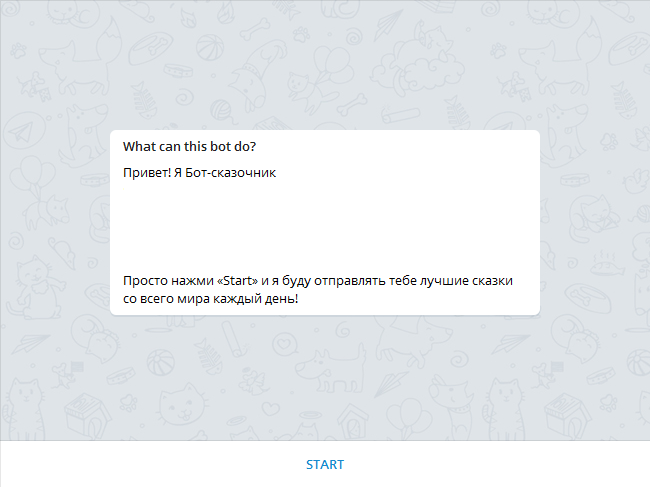
\includegraphics[width=\columnwidth]{./assets/y03s02-practice-01-report-p01.png}
					\caption{}
					\label{subfig:test-01}
				\end{subfigure}%
				\hspace{\baselineskip}%
				\begin{subfigure}[t]{0.5\textwidth-0.5\baselineskip}
					\centering
					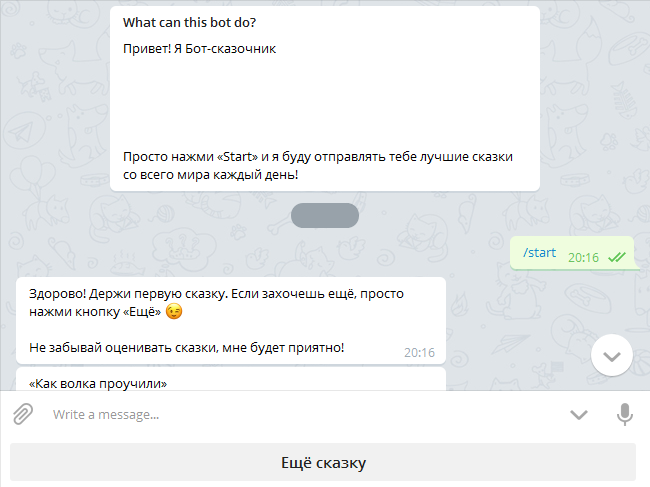
\includegraphics[width=\columnwidth]{./assets/y03s02-practice-01-report-p02.png}
					\caption{}
					\label{subfig:test-02}
				\end{subfigure}
				\begin{subfigure}[t]{0.5\textwidth-0.5\baselineskip}
					\centering
					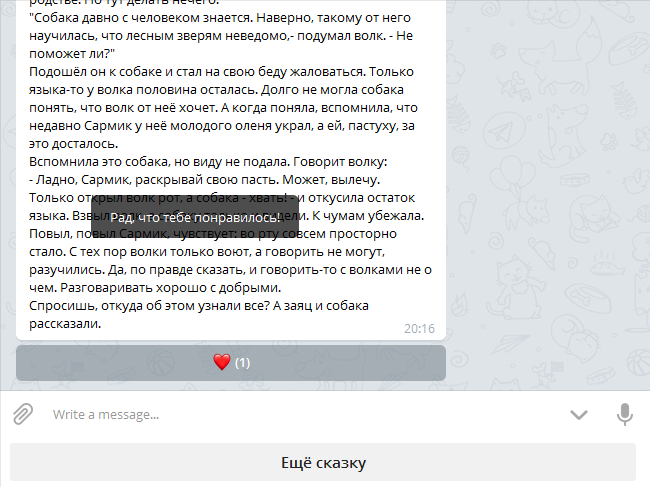
\includegraphics[width=\columnwidth]{./assets/y03s02-practice-01-report-p03.png}
					\caption{}
					\label{subfig:test-03}
				\end{subfigure}%
				\hspace{\baselineskip}%
				\begin{subfigure}[t]{0.5\textwidth-0.5\baselineskip}
					\centering
					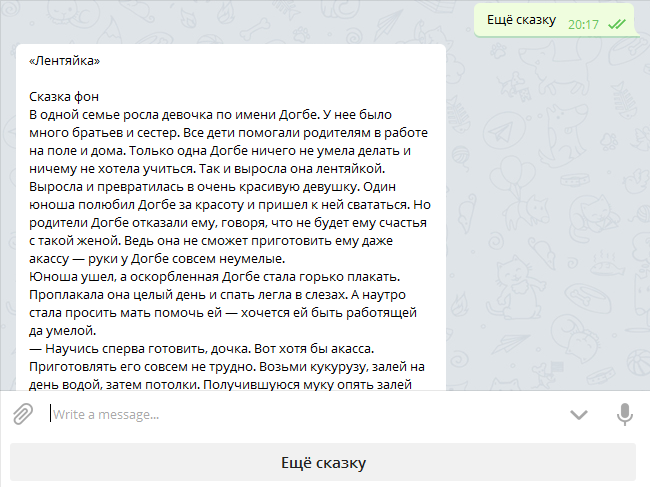
\includegraphics[width=\columnwidth]{./assets/y03s02-practice-01-report-p04.png}
					\caption{}
					\label{subfig:test-04}
				\end{subfigure}%
				\caption{Результати тестування чат-бота}
				\label{fig:test}
			\end{figure}

		\subsubsection{Результати}
			Розроблений програмний продукт був протестований. Тестування показало його правильну роботу і~готовність до~запуску.

	\section{Висновки}
		Проходячи проектно-технологічну практику в~організації~\allcaps{ТОВ}~«Смарт Медіа Інвест», я~розробив повноцінний прикладний програмний продукт~— чат-бота для~платформи~\textenglish{Telegram}, а~також протестував його.
		У~процесі розробки програмного продукту я~ознайомився з~процесом роботи розробника і~вдосконалив практичні навички роботи з~інфраструктурою, яка~використовується під~час життєвого циклу веб-додатків. На~базі практики її~складали такі елементи забезпечення:
		\begin{itemize}
				\item операційна система~\textenglish{\allcaps{GNU}/Linux Ubuntu \allcaps{LTS}};
				\item веб-сервер~\textenglish{Nginx};
				\item система керування базами даних~\textenglish{MongoDB};
				\item інтерпретатор мови програмування~\textenglish{Python};
				\item система управління контейнерами~\textenglish{Docker}.
		\end{itemize}
		Крім досвіду роботи з~інфраструктурою, я~покращив уміння розробки веб-додатків, а~також здобув досвід організації їх~взаємодії з~базами даних на~прикладі системи керування базами даних~\textenglish{MongoDB} і~її~інтерфейсу для~мови програмування~\textenglish{Python}~— пакету~\textenglish{PyMongo}.

		Розробивши продукт, я~використав платформу контейнеризації~\textenglish{Docker} для~розгортання продукту, що~дозволило вдосконалити навички налаштування і~запуску веб-додатків для~кінцевих користувачів. Після розробки рішення для~розгортання я~провів тестування продукту, яке показало, що~розроблений продукт справний і~готовий для~запуску для~кінцевих користувачів. За~результатами розробки база практики прийняла програмний продукт в~експлуатацію.

	\newpage
	\printbibliography[heading=bibintoc]

\end{document}

